\documentclass[UTF-8]{ctexart} 
\usepackage[a4paper,left=2cm,right=2cm,top=2.5cm,bottom=2.5cm]{geometry}
\usepackage{amsmath,bm,amssymb}
\usepackage{lmodern}
\usepackage{tikz}
\usepackage{wrapfig}
\usepackage{fancyhdr}
\usepackage{caption}
\usepackage{enumitem}
\usepackage{upgreek}
\usetikzlibrary{snakes}

\captionsetup{labelformat=empty}
%\renewcommand\thefigure{\theenumi}
\makeatletter
\renewcommand*\maketitle{
    \begin{center}
        \bfseries
        {\Large \@title \par}
        \vskip 1em
        {\global\let\author\@empty}
        {\global\let\date\@empty}
    \end{center}
  \setcounter{footnote}{0}
}
\newcommand\mlabel[2]{#2\def\@currentlabel{#2}\label{#1}}
\renewcommand\theenumi{S-\arabic{enumi}}
\renewcommand\labelenumi{\theenumi}
\makeatother

\pagestyle{fancy}
\fancyhf{}
\cfoot{\thepage}
\renewcommand\headrulewidth{0pt}
\title{第5章\ 静电场}
\author{叶旺全\\大学物理教研室}

\begin{document} 
\maketitle
\begin{enumerate}
    % \item[\mlabel{itm:a}{5-6}] 自定义label引用参考
    \item[5-7] 质量为\(m\),电荷为\(-e\)的电子以圆轨道绕氢核旋转,其动能为\(E_k\),
    证明电子的旋转频率满足
    \[
        v^2=\frac{32\varepsilon^2_0E^3_k}{me^4}
    \]
    式中\(\varepsilon_0\)是真空电容率。
    电子的运动可视为遵守经典力学定律。
    
    \item[5-10] 若电荷\(Q\)均匀地分布在长为\(L\)的细棒上,求证:
        \begin{enumerate}
            \item[(1)] 在棒的延长线上,且离棒中心为\(r\)处的电场强度为
                \[
                    E=\frac{1}{\uppi\varepsilon_0}\frac{Q}{4r^2-L^2}
                \]
            \item[(2)] 在棒的垂直平分线上,且离棒为\(r\)处的电场强度为
                \[
                    E=\frac{1}{2\uppi\varepsilon_0 r}\frac{Q}{\sqrt{4r^2+L^2}}
                \]
        \end{enumerate}
        若棒为无限长(即\(L\rightarrow\infty\)),试将结果与无限长均匀带电直导线的电场强度相比较。
    
    \item[5-11] 一半径为\(R\)的半球壳均匀地带有电荷,电荷面密度为\(\sigma\)。求球心处电场强度的大小。
    
    \item[5-13] 两根无限长平行直导线相距为\(r\),均匀带有等量异号电荷,电荷线密度为\(\lambda\)。
        (1) 求两导线构成的平面上任意一点的电场强度(设该点到其中一导线的垂直距离为\(x\));
        (2) 求一根导线上单位长度导线受到另一根导线上电荷作用的电场力。
    
    \item[\mlabel{itm:a}{5-16}] 如图所示,边长为\(a\)的立方体的表面分别平行于\(Oxy\)、\(Oyz\)和\(Ozx\)平面,
        立方体的一个顶点为坐标原点。现将立方体置于电场强度为\(\bm{E}=(E_1+kx)\bm{i}+E_2\bm{j}\)的非均匀电场
        中,求立方体各表面及立方体的电场强度通量(\(k\)、\(E_1\)、\(E_2\)均为常量)。
                       
        \begin{figure}[htbp]
            \centering
            \begin{minipage}[b]{.4\textwidth}
                \centering
                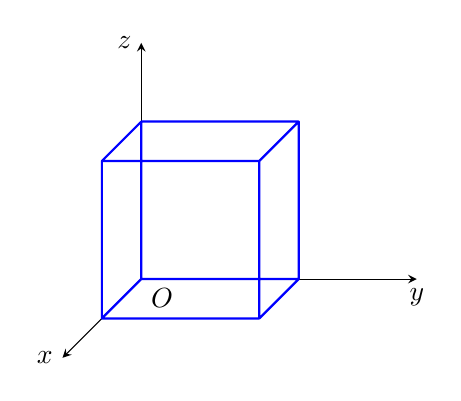
\begin{tikzpicture}
                    \draw[-stealth] (0,0) node[below right]{\(O\)} -- (3.5,0) node[below]{\(y\)};
                    \draw[-stealth] (0,0) -- (0,3) node[left]{\(z\)};
                    \draw[-stealth] (0,0) -- (-1,-1) node[left]{\(x\)};
                    \draw[join=round, blue, thick] (0,0) -- (2,0) -- (2,2) -- (0,2) --(0,0) --(-0.5,-0.5)
                        -- (1.5,-0.5) -- (1.5, 1.5) -- (-0.5,1.5) -- (0,2) -- (0,0) --(-0.5,-0.5)
                        -- (-0.5,1.5) -- (1.5, 1.5) -- (2,2) -- (2,0) -- (1.5,-0.5);
                \end{tikzpicture}
                \caption{\ref{itm:a} 题图}
            \end{minipage}
            \begin{minipage}[b]{.4\textwidth}
                \centering
                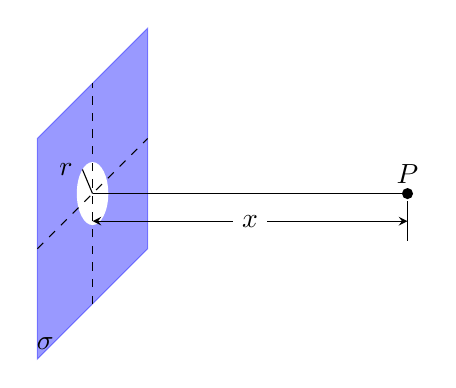
\begin{tikzpicture}
                    \filldraw[fill=blue,opacity=0.4,draw=blue] (0.7,2.1) -- (0.7,-.7) -- (-.7,-2.1) 
                        -- (-.7,.7) -- cycle;
                    \node at (-.6,-1.9) {\(\sigma\)};
                    \fill[fill=white] (0,0) ellipse (0.2 and 0.4);
                    \draw[dashed] (-0.7,-0.7) -- (0.7,0.7);
                    \draw[dashed] (0,-1.4) -- (0,1.4);
                    \draw[thin] (0,0) -- (130:0.2 and 0.4) node[left]{\(r\)};
                    \draw (0,0) -- (4,0);
                    \fill (4,0) circle (2pt) node[above]{\(P\)};
                    \draw (4,-0.1) -- (4,-0.6);
                    \draw[stealth-stealth] (4,-0.35) -- node[fill=white]{\(x\)} (0, -0.35);
                \end{tikzpicture}
                \caption{\ref{itm:b} 题图}
            \end{minipage}
        \end{figure} 


    \item[5-18] 设在半径为\(R\)的球体内,其电荷对称分布,电荷体密度为
        \[\begin{cases}
            \rho=kr, &0 \leqslant r \leqslant R\\
            \rho=0, &r>R
        \end{cases}\]
        式中\(k\)为一常量。试分别用高斯定理和电场叠加原理求电场强度\(\bm{E}\)与\(r\)的函数关系。
    
    \item[\mlabel{itm:b}{5-19}] 如图所示,一无限大均匀带电薄平板的电荷面密度为\(\sigma\)。在平板
        中部有一个半径为\(r\)的小圆孔。求圆孔中心轴线上与平板相距为\(x\)的一点\(P\)的电场强度。

    \item[\mlabel{itm:c}{5-20}] 如图所示,在电荷体密度为\(\rho\)的均匀带点球体中,存在一个球形空腔。
        如将带电体球心\(O\)指向球形空腔球心\(O^\prime\)的矢量用\(\bm{a}\)表示,试证明球形空腔中任意
        点的电场强度为
        \[
            \bm{E}=\frac{\rho}{3\varepsilon_0}\bm{a}
        \]
        \begin{figure}[htbp]
            \centering
            \begin{minipage}[b]{.4\textwidth}
                \centering
                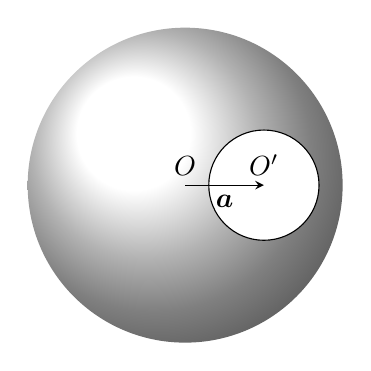
\begin{tikzpicture}
                    \shade[ball color=white] (0,0) circle(2);
                    \filldraw[fill=white] (1,0) circle(0.7); 
                    \draw[-stealth] (0,0) node[above]{\(O\)} -- node[below]{\(\bm{a}\)} (1,0) node[above]{\(O^\prime\)};
                \end{tikzpicture}
                \caption{\ref{itm:c} 题图}
            \end{minipage}
        \end{figure} 

    \item[5-23] 半径为\(R\)的无限长直圆柱体内均匀分布着电荷,电荷体密度为\(\rho\)。试求离轴线为\(r\)
        处的电场强度\(\bm{E}\),并画出\(E-r\)曲线。

    \item[\mlabel{itm:d}{5-25}] 如图所示,三个点电荷\(Q_1\)、\(Q_2\)、\(Q_3\)沿一条直线等间距分布,且\(Q_1=Q_3=Q\)。
        已知其中任一点电荷所受合力均为零,求在固定\(Q_1\)、\(Q_3\)的情况下,将\(Q_2\)从点\(O\)移到无穷远处
        外力所做的功。
        \begin{figure}[htbp]
            \centering
            \begin{minipage}[b]{.4\textwidth}
                \centering
                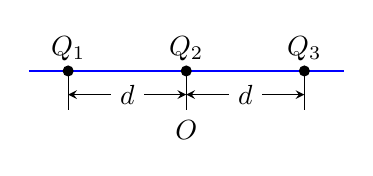
\begin{tikzpicture}
                    \draw[blue,thick] (-2,0) -- (2,0);
                    \foreach \x in {1,2,3}
                    {
                        \fill (\x * 1.5-3,0) circle(2pt) node[above]{\(Q_\x\)};
                        \draw (\x * 1.5-3,0) -- +(0,-0.5);
                    }
                    \draw[stealth-stealth][yshift=-0.3cm] (-1.5,0) -- node[fill=white]{\(d\)} (0,0);
                    \draw[stealth-stealth][yshift=-0.3cm] (0,0) -- node[fill=white]{\(d\)} (1.5,0);
                    \node[below] at (0,-0.5) {\(O\)};
                \end{tikzpicture}
                \caption{\ref{itm:d} 题图}
            \end{minipage}
        \end{figure} 
        
    \item[5-28] 一个球形雨滴半径为0.40\,mm,带有电荷量1.6\,pC,它表面的电势有多大?两个这样的雨滴
        相遇后合并为一个较大的雨滴,这个雨滴表面的电势又是多大?

    \item[5-31] 两个同心球面的半径分别为\(R_1\)和\(R_2\),各自带有电荷\(Q_1\)和\(Q_2\)。求:
        (1)各区域电势的分布,并画出分布曲线;(2)两球面上的电势差。
    
    \item[5-33] 一圆盘半径\(R=3.00\times10^{-2}\, \mathrm{m}\),圆盘均匀带电,电荷面密度\(\sigma=2.00\times10^{-5}\,\mathrm{C\cdot m^{-2}}\)。
        (1)求轴线上的电势分布;(2)根据电场强度和电势梯度的关系求电场分布;(3)计算离盘心30.0\,cm处的电势
        和电场强度。
    
    \item[5-34] 两根同长的同轴圆柱面(\(R_1=3.00\times10^{-2}\, \mathrm{m}, R_2=0.10\,\mathrm{m}\),带有等量异号的电荷,
        两者的电势差为450\,V。求:(1)圆柱面单位长度所带的电荷;(2)\(r=0.05\,\mathrm{m}\)处的电场强度。
    
    \item[\mlabel{itm:e}{5-39}] 如图所示,在\(Oxyz\)平面上倒扣着半径为\(R\)的半球面,在半球面上电荷均匀分布,其电荷面密度为\(\sigma\)。点\(A\)的
        坐标为\((0,R/2)\),点\(B\)的坐标为\((3R/2,0)\),求电势差\(U_{AB}\)。
        \begin{figure}[htbp]
            \centering
            \begin{minipage}[b]{0.4\textwidth}
                \centering
                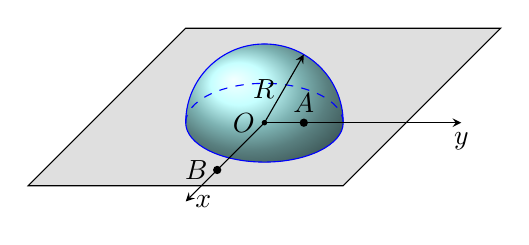
\begin{tikzpicture}
                    \filldraw[fill=lightgray!50,draw=black] (1,-0.8) -- (3,1.2) -- (-1,1.2) -- (-3,-0.8) -- cycle;
                    \fill[ball color=cyan!30] (0:1) arc (0:180:1) arc (180:360:1 and 0.5);
                    \draw[blue] (0:1) arc (0:180:1) arc (180:360:1 and 0.5);
                    \draw[join=round,dashed,blue,] (0:1 and 0.5) arc (0:180:1 and 0.5);
                    \draw[-stealth] (0,0) node[left]{\(O\)} -- node[left]{\(R\)} (60:1);
                    \draw[-stealth] (0,0) -- (2.5,0) node[below]{\(y\)};
                    \draw[-stealth] (0,0) -- (-1,-1) node[right]{\(x\)};
                    \fill (-0.6,-0.6) circle(1.5pt) node[left]{\(B\)};
                    \fill (0.5,0) circle(1.5pt) node[above]{\(A\)};
                    \fill (00,0) circle(1pt);
                \end{tikzpicture}
                \caption{\ref{itm:e} 题图}
            \end{minipage}
        \end{figure}
    
    \item[5-40] 在玻尔的氢原子模型中,电子沿半径为\(0.53\times10^{-10}\,\mathrm{m}\)的圆周绕原子核旋转。
        (1)若把电子从原子中拉出来,则需要克服电场力做多少功?(2)电子的电离能为多少?
        % \begin{figure}[htbp]
        %     \centering
        %     \begin{minipage}[b]{.4\textwidth}
        %         \centering
        %         \begin{tikzpicture}[scale=0.5]
        %             \draw[decorate,decoration={bumps,mirror,segment length=19 pt}] (0:0) circle(3);
        %             \draw (0,0) circle(2.8);
        %             \foreach \x in {0,20,...,340}
        %             {
        %                 \draw[rotate=\x] (1.3,0) ellipse(1.3 and 0.3);
        %             }
        %             \filldraw[fill=white,rounded corners=1.5ex] (-1.6,0.8) rectangle (1.6,-0.8);
        %             \node at (0,0) {\Large \textbf{保过}};
        %         \end{tikzpicture}
        %         \caption{月饼}
        %     \end{minipage}
        % \end{figure}
    \item \label{itm:1} 有一边长为\(a\)的正方形平面,在其中垂线上距中心\(O\)点\(\frac{a}{2}\)处,
    有一电荷量为\(q\)的正点电荷,如图,则通过该平面的电场强度通量为多少? 
    \textit{\small(利用高斯定理求解)}     
    
        \begin{figure}[htb]
            \centering
            \begin{minipage}[b]{0.4\textwidth}
                \centering
                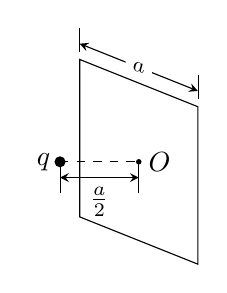
\begin{tikzpicture}
                    \newcommand\drawit{\draw[xscale = 0.75, yslant=-0.3]}
                    \drawit (-1,-1) rectangle(1,1);
                    \coordinate[label=right:\(O\)] (O) at (0,0);
                    \fill (-1,0) circle(2pt);
                    \fill (0,0) circle(1pt);
                    \coordinate[label=left:\(q\)] (q) at (-1,0);
                    \draw[dashed] (q) -- (O);
                    \draw[very thin] (-1,-0.4) -- (q);
                    \draw[very thin] (0,-0.4) -- (O);
                    \draw[stealth-stealth] (-1,-0.2) -- (0,-0.2) ;
                    \node[below] at (-0.5,-0.2) {\(\frac a2\)};
                    \drawit[very thin] (-1,1.1) -- (-1,1.4);
                    \drawit[very thin] (1,1.1) -- (1,1.4);
                    \drawit[stealth-stealth] (-1,1.2) -- (1,1.2) ;
                    \node[fill=white, yslant=-0.3, scale = 0.8] at (0,1.2) {\(a\)};
                \end{tikzpicture}
                \caption{\ref{itm:1} 题图}
            \end{minipage}
            \begin{minipage}[b]{0.4\textwidth}
                \centering
                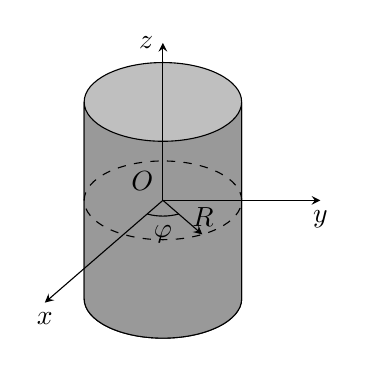
\begin{tikzpicture}
                    \def\myel{1 and 0.5};
                    \filldraw[fill=black!25,draw=black] (0:\myel) +(0,1.25) arc (0:180:\myel) 
                        -- +(0,-2.5) arc (180:360:\myel) -- cycle;
                    \filldraw[fill=black!40,draw=black] (0:\myel) +(0,1.25) arc (0:-180:\myel) 
                        -- +(0,-2.5) arc (180:360:\myel) -- cycle;
                    \draw[dashed] (0,0) ellipse (1 and 0.5);
                    \draw[-stealth] (0,0) node[above left]{\(O\)} -- (2,0) node[below]{\(y\)};
                    \draw[-stealth] (0,0) -- (0,2) node[left]{\(z\)};
                    \draw[-stealth] (0,0) -- (240:3 and 1.5) node[below]{\(x\)};
                    \draw[-stealth] (0,0) -- node[right]{\(R\)} (300:\myel);
                    \draw (240:0.4 and 0.2) arc (240:300:0.4 and 0.2) node[below,midway]{\(\varphi\)} ;
                \end{tikzpicture}
                \caption{\ref{itm:3} 题图}
            \end{minipage}
        \end{figure}

    \item \label{itm:2} 如图,无限长带电半圆柱面的电荷面密度为\(\sigma\)。试求圆柱轴线(点划线)上的电场强度。
    
        \begin{figure}[htb]
            \centering
            \begin{minipage}[b]{0.4\textwidth}
                \centering
                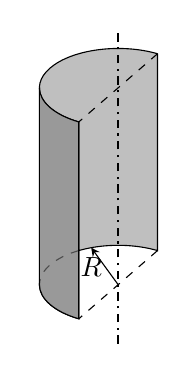
\begin{tikzpicture}
                    \def\myel{1 and 0.5};
                    \filldraw[fill=black!25,draw=black] (60:\myel) +(0,2.5) arc (60:240:\myel) 
                    -- (240:\myel) arc (240:60:\myel) -- +(0,2.5);
                    \filldraw[fill=black!40,draw=black] (180:\myel) +(0,2.5) arc (180:240:\myel) 
                    -- (240:\myel) arc (240:180:\myel) -- +(0,2.5);
                    \draw[dashed,opacity=0.5] (120:\myel) arc (120:180:\myel);
                    \draw[dashed] (0,2.5) +(60:\myel) -- +(240:\myel);
                    \draw[dashed] (60:\myel) -- (240:\myel);
                    \draw[thick, dash dot] (0,-0.75) -- (0,3.25);
                    \draw[-stealth] (0,0) -- (110:\myel) node[below]{\(R\)};
                \end{tikzpicture}
                \caption{\ref{itm:2} 题图}
            \end{minipage}
            \begin{minipage}[b]{0.4\textwidth}
                \centering
                \begin{tikzpicture}
                    \draw (0,0) ellipse(1 and 2);
                    \node[anchor=north west] at (135:1 and 2) {\(\lambda_1\)};
                    \draw (0,0) -- (2,0) node[below]{\(\lambda_2\)};
                    \draw[dashed] (2,0) -- (4,0);
                    \draw[dashed, -stealth] (0,0) node[above]{\(O\)} -- (200:1 and 2) node[midway,below]{\(R\)};
                \end{tikzpicture}
                \caption{\ref{itm:4} 题图}
            \end{minipage}
        \end{figure}
    \item \label{itm:3} 一“无限长”圆柱面,其电荷面密度为:\(\sigma=\sigma_0\cos \varphi\)(\(\sigma_0\)为常数),
    其中\(\varphi\)为半径\(R\)与\(x\)轴所夹的角,试求圆柱轴线(\(z\)轴)上任意一点的场强。
    
    \item 半径为\(R\)的无限长直圆柱体内均匀分布着电荷,电荷体密度为\(\rho\)。试求离轴线为\(r\)
        处的电势\(V\),并画出\(V-r\)曲线(取圆柱表面为电势零点)。
    
    \item \label{itm:4} 如图所示,半径为\(R\)的均匀带电细圆环电荷线密度为\(\lambda_1\),在圆环的轴线上有一无限长均匀带电直线,
        电荷线密度为\(\lambda_2\),直线的一个端点正好处于圆环的圆心上,设圆环对直线电荷的分布没有影响,
        求圆环对直线的作用力。
    
    \item 分别绘制半径为\(R\)的(1)均匀带电球体;(2)均匀带电球壳以及(3)带等量异号电荷(\(-q,+q\))的
        半径分别为\(R_1\)和\(R_2\)的同心球壳(\(R_1<R_2\))的\(E-r\)、\(V-r\)曲线。
\end{enumerate}
\end{document} 